\chapter{Conclusioni}\label{cap:conclusioni}
\section{Conclusioni}\label{sez:conclusioni}
Questo studio, ha cercato di rispondere alla domanda: "Cos'\`e Blazor?".
A tal fine, \`e stato descritto prima di tutto quali siano le tecnologie utilizzate da questo framework che in parte cambiano a seconda del modello scelto.
\`E stata implementata una applicazione web sfruttando Blazor Server, e dove disponibili sono stati mostrati gli esempi disponibili per gli altri modelli.
Ci\`o \`e stato fatto per spiegare il diverso funzionamento, a seconda del modello scelto, con i pro e contro di ciascuno.
\`E emerso che non esiste una scelta universalmente giusta, poich\'e a seconda delle esigenze dell'applicazione da sviluppare, un modello pu\`o risultare pi\`u o meno adatto.

\section{Futuro del progetto}\label{sez:futuro}
\begin{figure}[H]
	\centerline{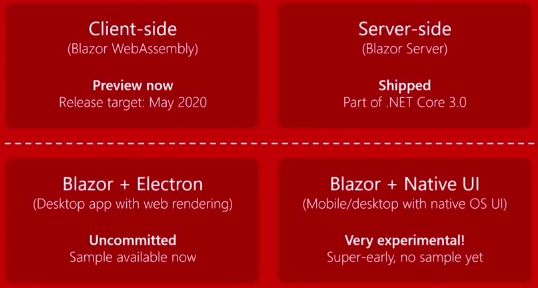
\includegraphics[scale=0.8]{figure/ModelsSupportedOrNot.png}}
	\caption{Modelli blazor e supporto}
	\label{fig:supportedBlazorModels}
\end{figure}

\begin{figure}[H]
	\centerline{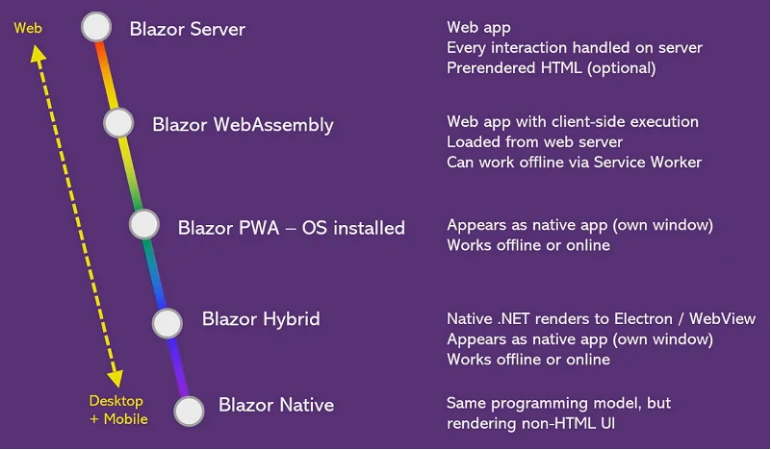
\includegraphics[scale=0.6]{figure/BlazorModels.PNG}}
	\caption{Modelli attuali e futuri}
	\label{fig:blazorModels}
\end{figure}

Onbeforeunload

Server 

WebAssembly, promettente ma ancora interpretato, si dovrebbe tradurre .NET direttamente in WebAssembly e in modalità AOT per avere prestazioni ben migliori e giustificare il non utilizzo di JS.

In Roadmap
PWA solo su Chrome
Electron, bello ma molto pesante
Native --> la complessità non giustifica la scelta, al momento e un esercizio accademico.